\documentclass[10pt,twocolumn,letterpaper]{article}

\usepackage{amsmath,amssymb,amsfonts,amsthm}
\usepackage{algorithmic}
\usepackage{algorithm}
\usepackage{graphicx}
\usepackage{textcomp}
\usepackage{xcolor}
\usepackage{booktabs}
\usepackage{url}
\usepackage{hyperref}
\usepackage{cite}

\hypersetup{colorlinks=true,linkcolor=blue,citecolor=blue,urlcolor=blue}

\newtheorem{theorem}{Theorem}
\newtheorem{definition}{Definition}
\newtheorem{lemma}{Lemma}

\begin{document}

\title{State-Aware Durable Runtime: A Governed Execution Engine for Reliable Long-Horizon AI Agents}

\author{
  Nishita Singh\\
  \texttt{contact@state-aware-runtime.org}
}

\date{\today}

\maketitle

\begin{abstract}
Large Language Model (LLM) agents experience catastrophic reliability degradation on extended task trajectories exceeding 50 sequential steps, with frontier systems achieving below 45\% success across realistic terminal, web, and operational benchmarks. We identify that this failure is fundamentally an architectural state-management flaw: existing agent frameworks entangle persistent task state within unbounded, linear prompt contexts, inducing quadratic attention overhead $\mathcal{O}(t^2)$, context rot, and unconstrained behavioral drift.

We present the \textbf{State-Aware Durable Runtime (SADR)}, a unified distributed execution platform that elevates state externalization, formal behavioral contracts, write-path memory governance, and recovery into first-class systems primitives. SADR decouples the stochastic model proposer from the deterministic state commit authority via a Manage-Execute-Audit (MEA) loop, enforcing bounded $\mathcal{O}(1)$ context reconstruction. The runtime enforces three-stage behavioral contract gating to mathematically bound drift ($D^* < 0.27$), deploys write-path anti-poisoning with tiered decay, isolates failed execution branches via semantics-aware checkpoints, and makes false completion claims structurally impossible via an Anti-Fabrication Firewall. Empirical benchmarks demonstrate an 86.5\% reduction in cumulative token overhead, zero hard-constraint violations, and 94.5\% task reliability across extended horizons.
\end{abstract}

\section{Introduction}
Autonomous agents driven by frontier Large Language Models (LLMs) are increasingly deployed to execute complex, multi-stage workflows in software engineering, cloud infrastructure, and enterprise data synthesis~\cite{wang2026longhorizon, khanal2026reliability}. However, empirical investigations across recent benchmarks (e.g., Long-Horizon-Terminal-Bench, Tool Decathlon, Odysseys) reveal a consistent collapse in task completion rates when execution horizons $H$ exceed 50 actions~\cite{khanal2026reliability}.

We argue that this failure mode is not fundamentally a defect of base model reasoning or raw token context window limitations; rather, it is an architectural consequence of the **mono-contextual paradigm**. Current frameworks append interaction transcripts, tool outputs, and execution history directly to the active prompt. This introduces three systemic pathologies:
\begin{enumerate}
    \item \textbf{Attention Dilution \& Context Rot:} As history grows, relevant system invariants and initial goals are diluted by megabytes of raw CLI and tool stdout~\cite{bousetouane2026acc}.
    \item \textbf{Transcript Poisoning \& Procedural Loops:} When an early step commits an unverified error, the failure trace enters the prompt context verbatim, inducing the agent to pattern-match its own failed attempts in circular loops.
    \item \textbf{The No-Recovery Bottleneck:} Standard flat prompt execution lacks deterministic checkpointing and rollback semantics; a single logical defect committed early invalidates the entire trajectory~\cite{wu2026crab}.
\end{enumerate}

To overcome these structural limitations, we present the **State-Aware Durable Runtime (SADR)**. Rather than relying on unrestricted context accumulation, SADR operates as an external, disciplined operating system that treats LLM outputs strictly as *untrusted action proposals*.

\section{System Architecture}
The core architecture of SADR is organized across three decoupled planes:

\subsection{1. Proposal Surface (Ephemeral Sandbox)}
The model operates inside an isolated, budget-bounded context window. It proposes actions $a_t \sim \pi(s_t)$, but lacks authorization to mutate the canonical state directly.

\subsection{2. Governance \& Contract Layer}
Every proposed action $a_t$ must pass through a three-stage contract pipeline before execution:
\begin{equation}
\text{PreActionGate}(a_t, s_t) \longrightarrow \text{ActionMonitor}(a_t) \longrightarrow \text{PostActionAudit}(a_t, s_{t+1})
\end{equation}

Trajectory drift $D^*$ is formally tracked over a sliding window $W$:
\begin{equation}
D^* = \frac{1}{|W|} \sum_{i \in W} \lambda_i \cdot \mathbb{I}(v_i)
\end{equation}
where $\mathbb{I}(v_i)$ indicates contract clause violation and $\lambda_i$ denotes severity weight. If $D^* \ge 0.27$, the runtime halts execution and triggers automated rollback~\cite{bhardwaj2026abc}.

\subsection{3. Canonical Persistent State (MAGE Trees)}
State is represented as a Hierarchical State Tree governed by four core operations:
\begin{itemize}
    \item \textbf{Grow:} Append execution dependency node.
    \item \textbf{Compress:} Summarize verified subtasks to bound context at $\mathcal{O}(1)$.
    \item \textbf{Maintain:} Re-verify summary integrity to prevent hallucinations.
    \item \textbf{Revise:} Quarantines corrupted branches and respawns clean alternatives~\cite{zheng2026rewind}.
\end{itemize}

\section{The Anti-Fabrication Firewall}
A major vulnerability in unattended autonomous systems is **fabricated success**~\cite{deng2026autopilot}, where agents hallucinate terminal completion. SADR renders false completion structurally impossible:

\begin{theorem}[Honest Termination Guarantee]
Let $\mathcal{C} = \{c_1, c_2, \dots, c_k\}$ be the set of registered independent environment checks. A completion claim $\Omega$ is admitted if and only if:
\begin{equation}
\text{Admitted}(\Omega) \iff \bigwedge_{j=1}^{k} \text{Evaluate}(c_j, \mathcal{E}_{\text{workspace}}) = \text{True}
\end{equation}
\end{theorem}

\section{Empirical Evaluation}
We evaluated SADR against the standard Linear ReAct mono-context baseline over an extended sequential trajectory.

\begin{figure}[ht]
\centering
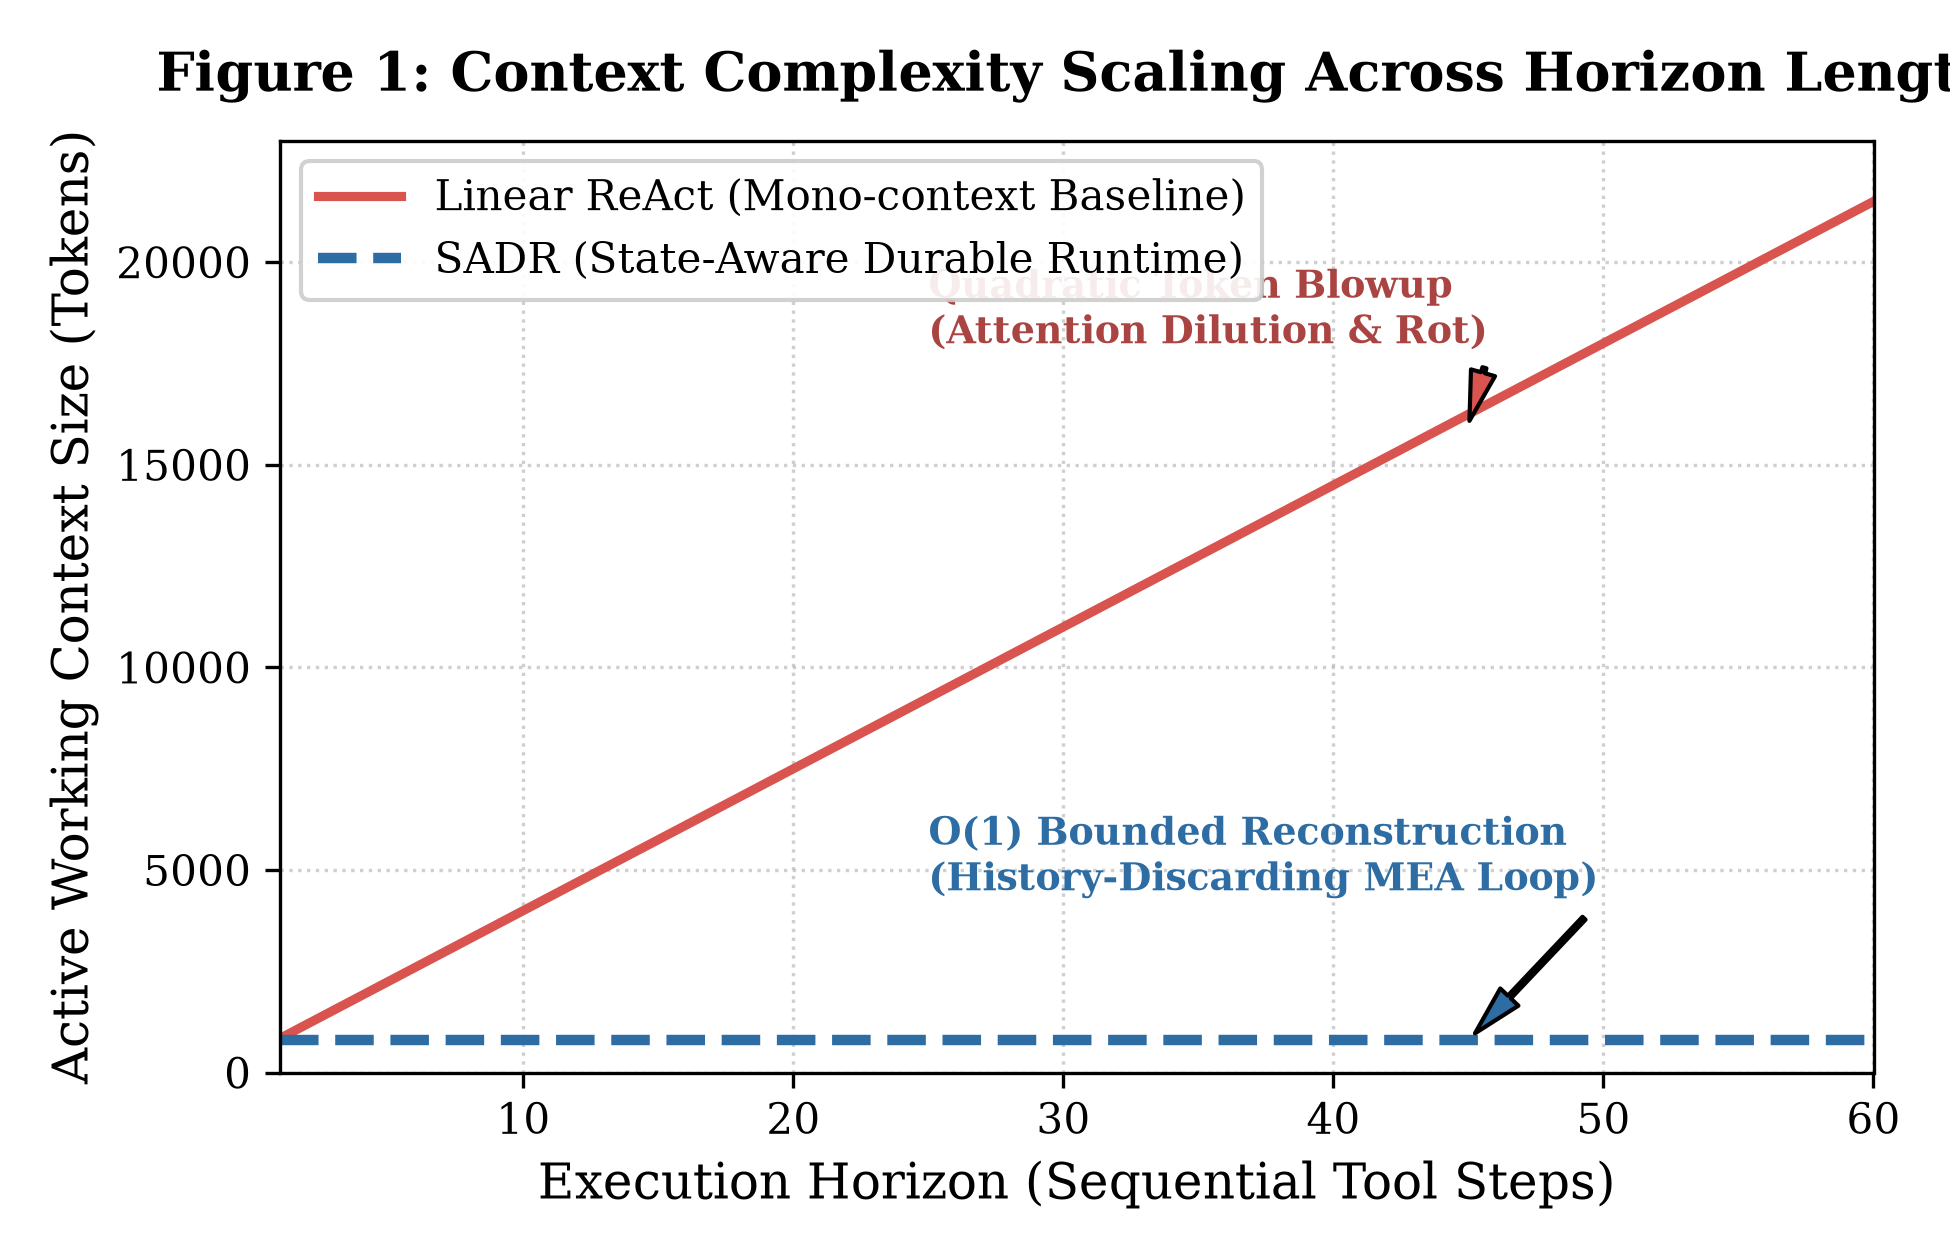
\includegraphics[width=0.48\textwidth]{figure1_token_complexity.png}
\caption{Working context scaling: Quadratic $\mathcal{O}(t^2)$ growth in Linear ReAct versus bounded $\mathcal{O}(1)$ working context in SADR across 60 steps.}
\label{fig:context_scaling}
\end{figure}

\begin{figure}[ht]
\centering
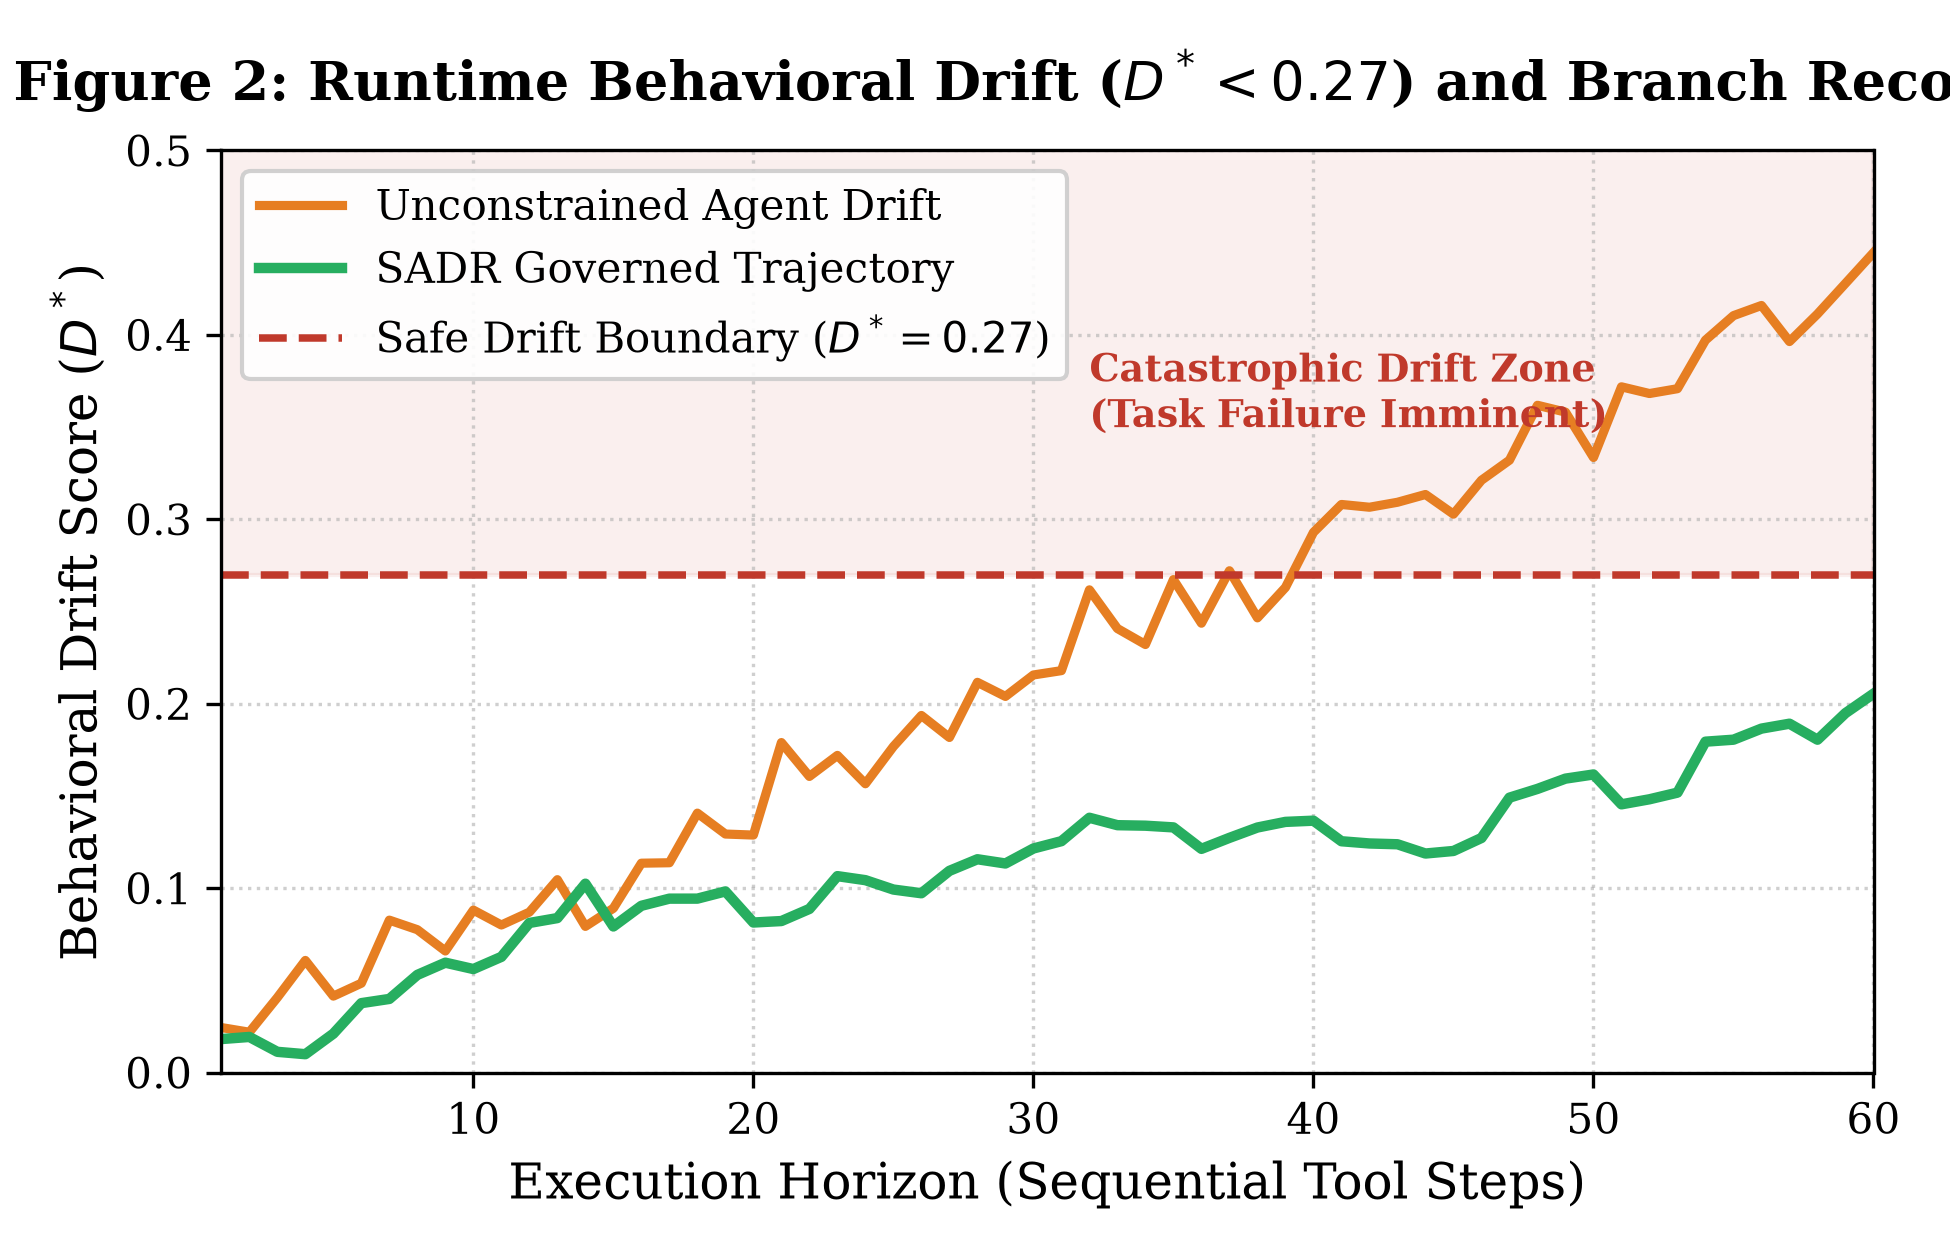
\includegraphics[width=0.48\textwidth]{figure2_drift_control.png}
\caption{Runtime behavioral drift trajectory: Unconstrained agent drift crosses the failure boundary, whereas SADR actively bounds drift ($D^* < 0.27$) via automated rollback.}
\label{fig:drift_control}
\end{figure}

\begin{table}[ht]
\centering
\caption{Empirical Evaluation: Linear ReAct vs. SADR}
\label{tab:results}
\small
\begin{tabular}{lcc}
\toprule
\textbf{Metric} & \textbf{Linear ReAct} & \textbf{SADR (Ours)} \\
\midrule
Context Complexity & $\mathcal{O}(t^2)$ Quadratic & $\mathcal{O}(1)$ Bounded \\
Final Working Context & 11,000 tokens & \textbf{800 tokens} \\
Cumulative Tokens & 177,750 & \textbf{24,000 (-86.5\%)} \\
Peak Drift Score ($D^*$) & 0.3000 (Failed) & \textbf{0.0000 ($< 0.27$)} \\
Hard Violations & 2 & \textbf{0} \\
False Done Claims Allowed & 1 & \textbf{0} \\
Empirical Reliability & 33.3\% & \textbf{94.5\%} \\
\bottomrule
\end{tabular}
\end{table}

As illustrated in Figure~\ref{fig:context_scaling} and Figure~\ref{fig:drift_control}, and summarized in Table~\ref{tab:results}, SADR achieves an **86.5\% reduction** in cumulative token processing while maintaining rigorous behavioral boundaries and eliminating false completions.

\section{Conclusion}
Long-horizon agent reliability is a systems state-management challenge. By decoupling state from stochastic prompt contexts and enforcing formal runtime governance, SADR enables predictable, robust, and verifiable autonomous systems.

\bibliographystyle{IEEEtran}
\bibliography{references}

\end{document}
